The given equation can be written as,
\begin{align}
    \vec{x}^T\myvec{4 & 0 \\ 0 & 0}\vec{x} + \myvec{3 & 0}\vec{x} + 5 = 0 \label{2/19/eq:1}
\end{align}
where,
\begin{align}
    \vec{x} = \myvec{x \\ 0} \label{2/19/eq:2}
\end{align}
Substituting \eqref{2/19/eq:2} in \eqref{2/19/eq:1},
\begin{align}
    \myvec{x & 0}\myvec{4 & 0 \\ 0 & 0}\myvec{x \\ 0} + \myvec{3 & 0}\myvec{x \\ 0} + 5 &= 0 \\
    \implies 4x^2 + 3x + 5 &= 0\\
    \implies \brak{2x + \frac{3}{4}}^2 &= -\frac{71}{16}\label{2/19/eq:3}
\end{align}
The square of a real number is always non-negative. In \eqref{2/19/eq:3}, we can say that $2x + \frac{3}{4}$ is not a real number. So, the roots are not real. From the figure, we can see that the function does not cross the x-axis, so, the quadratic equation has no real roots. Obtaining the affine transformation,
\begin{align}
    \vec{V} &= \myvec{4 & 0 \\ 0 & 0}\\
    \vec{u} &= \myvec{\frac{3}{2}\\\frac{-3}{2}}\\
    f &= 5
\end{align}
The equation used for affine transformation
\begin{align}
    \vec{x} = \vec{P}\vec{y} + \vec{c}
\end{align}
The eigenvalues of $V$ are
\begin{align}
    \lambda_1 = 4\\
    \lambda_2 = 0\\
    \vec{D} = \myvec{4 & 0\\0 & 0}
\end{align}
The eigenvectors of $V$ are
\begin{align}
    \vec{p}_1 &= \myvec{0 \\ 1}\\
    \vec{p}_2 &= \myvec{1 \\ 0}\\
    \vec{P} &= \myvec{\vec{p}_1 & \vec{p}_2}\\
    &= \myvec{0 & 1 \\ 1 & 0}
\end{align}
Since $|\vec{V}| = 0$,
\begin{align}
    \myvec{\vec{u}^T+\eta \vec{p}_1^T \\ \vec{V}}\vec{c} &= \myvec{-f \\ \eta \vec{p}_1-\vec{u}}\\
    \eta &= \vec{u}^\top \vec{p}_1\\
    \implies \eta &= -\frac{3}{2}\\
    \implies \myvec{\frac{3}{2} & -3 \\ 4 & 0 \\ 0 & 0}\vec{c} &= \myvec{-5 \\ -\frac{3}{2} \\ 0}\\
    \implies \vec{c} &= \myvec{\frac{-3}{8}\\\frac{71}{48}}
\end{align}
The quadratic equation will not have real roots if
\begin{align}
    \brak{\vec{p_1}^T\vec{c}}\brak{\vec{p_2}^T\vec{V}\vec{p_2}} > 0
\end{align}
Substituting the values in LHS,
\begin{align}
    \brak{\vec{p_1}^T\vec{c}}\brak{\vec{p_2}^T\vec{V}\vec{p_2}} &= \brak{\frac{71}{48}}\brak{4}\\
    &= \frac{71}{12}
\end{align}
Since the value is positive, the quadratic equation has no real roots. Finding the roots of the equation. The equation of line is,
\begin{align}
    L : \vec{x} = \vec{q} + \mu\vec{m}, \mu \in \mathbb{R}
\end{align}
The line $L$ is the x-axis,
\begin{align}
    \vec{q} = \myvec{0 \\ 0}\\
    \vec{m} = \myvec{1 \\ 0}
\end{align}
The line $L$ intersects the conic and to find $\mu$,
\begin{multline}
    \mu = \frac{-\vec{m}^T \brak{\vec{V}\vec{q} + \vec{u}}}{\vec{m}^T\vec{V}\vec{m}} \pm \\ \frac{\sqrt{\brak{\vec{m}^T\brak{\vec{V}\vec{q} + \vec{u}}}^2 - \brak{\vec{q}^T\vec{V}\vec{q} + 2\vec{u}^T\vec{q} + f}\brak{\vec{m}^T\vec{V}\vec{m}}}}{\vec{m}^T\vec{V}\vec{m}}
\end{multline}
\begin{align}
    \mu &= \frac{-3}{8} \pm \frac{\sqrt{-71}}{8}\\
    &= \myvec{\frac{-3}{8} \\ \frac{\sqrt{71}}{8}}, \myvec{\frac{-3}{8} \\ \frac{-\sqrt{71}}{8}}
\end{align}
So, the roots of the equation are $\myvec{\frac{-3}{8} \\ \frac{\sqrt{71}}{8}}, \myvec{\frac{-3}{8} \\ \frac{-\sqrt{71}}{8}}$.
\begin{figure}[htp]
    \centering
    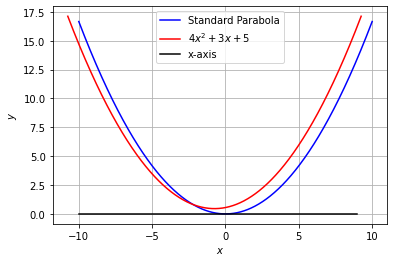
\includegraphics[width=\columnwidth]{solutions/oct/2/19/Figures/Fig1.png}
    \caption{Plot of the function}
    \label{2/19/fig:plot}
\end{figure}
